\documentclass[a4paper,11pt,pdf]{pacmanreport}

%%=== Aditional packages
%\usepackage{natbib}
%\setcitestyle{round}
% The following is used to make packages hyperref and cite work together
\makeatletter
\let\NAT@parse\undefined
\makeatother
\usepackage[bookmarks=true,hyperfootnotes=true,colorlinks=true,linkcolor=blue,anchorcolor=blue,citecolor=blue,urlcolor=blue,filecolor=blue]{hyperref}

%%=== Local definitions
\graphicspath{{images/}{../shared_images/}}

%% ================================
%% PROJECT INFO

\project{}
\projectid{FP7-IST-60918}
\projectstart{1 March 2013}
\duration{36}

%% ================================
%% DELIVERABLE INFO

\title{Multi-modal compositional hierarchies}
\deliverableid{DR 2.1}
\author{M. Popa, S. Rezapour-Lakani, A. Rietzler, F. Spinelli, C. J. Rosales, J. Piater}
\address{Institute of Computer Science, University of Innsbruck}
\email{Mirela.Popa@uibk.ac.at}
\headertitle{Multi-modal compositional hierarchies}
\headerauthor{M.~Popa et al}

\duedate{2015-02-28}
\submissiondate{2015-02-28}
\leadpartner{UIBK}
\revision{final}
\disseminationlevel{PU}


%% UNCOMMENT: to get the logo; if you've copied this file to a directory yearX/wpY/ then this should work
\reportlogo{pacmanlogo}


\begin{document}

\maketitle

\begin{abstract}
\noindent This deliverable describes the intermediate results of Tasks 2.1 and 2.2 as specified in the DoW. In this report the representations of shape and the inference methods developed are described along with the way in which grasps are attached to the object representations.
\end{abstract}

\vspace{.2em}
\hrule

\footnotesize

\tableofcontents

\normalsize

\newpage

\section*{Executive Summary}

This report presents work carried out in WP2 on multi-modal compositional hierarchies of object categories, using both visual and non-visual features. The 
work addresses the intermediate results of Tasks 2.1, 2.2 and 2.3. We describe 
an approach for integrating non-visual features into the compositional 
hierarchy, as defined in Task 2.1.
%, which is presented in detail in Annex \ref{ann:techReport}.

Next, we present the association of graspability to object parts formed using a hhierarchical representation, according to Task 2.2. In addition, we propose a 
method for structuring compositional object models into semantically meaningful 
parts, guided by their graspability.
%, which is described in a submitted conference paper included in Annex \ref{ann:icvs}.

\section*{Role of the Multi-modal compositional hierarchies in PaCMan}

In WP2, we focus on integrating non-visual features into the multi-modal compositional hierarchy. compositional hierarchy. Furthermore, we propose forming semantically meaningful parts based on their functionality. Both these aspects contribute to a better 
understanding of the environment and  will be used to refine object hypothesis, 
decompose an object into graspable parts, as well as reasoning under incomplete 
observations, either visual or non-visual.


\section*{Contribution to the PaCMan scenario}

information and to support reasoning under uncertainty in the 
dishwasher-scenarios addressed in WP5. Furthermore, by using the algorithms 
described in this report, a scene can be analyzed in a refined manner, by 
extracting information not only about object classes, but also about the 
semantically meaningful object parts and their graspability property. Moreover, 
the analysis of the non-visual information, such as tactile information can be 
used to analyze to success of an object grasp.

\newpage

\section{Tasks, objectives, results}

The objective of WP2 address the integration of visual and non-visual modalities 
into a single representation. The obtained unified, rich, compositional 
representation that incorporates complementary modalities, namely, visual 
features, as well as non-visual features will allow inference of unobserved from 
observed modalities, joint consideration of distinct modalities for increased 
robustness, and generalization to novel objects via shared parts.

\subsection{Planned work}

DR 2.1 addresses multi-modal compositional hierarchies for object representation using both visual and non-visual information. 

Planned work for each Task in WP2 is as follows:
\begin{enumerate}

\item[] \textbf{Task 2.1} The objective of Task 2.1 consists of integration of 
non-visual features into the compositional model, by defining a suitable 
parametrization of haptic features. Next, it addresses the development of 
methods for incremental acquisition of haptic information and its incorporation 
into the multi-modal representation. 

\item[] \textbf{Task 2.2} refers to the integration of graspability into the 
compositional 3D model, by associating grasps to object parts learned using a 
compositional approach.

\item[] \textbf{Task 2.3} In Task 2.3, algorithms for structuring the 3D 
compositional models based on graspability are designed and implemented.

\item[] \textbf{Task 2.4} addresses the detailed description of a scene, using 
all types of information provided by the multi-modal representation, such as 
object models described by their pose, as well as any visual, haptic and 
graspability properties associated with the objects.

\end{enumerate}

\subsection{Actual work performed}

In this section, the main achievements related to the topic of this deliverable are briefly described.
%For detailed descriptions of the work performed, the reader is referred to the papers and technical reports in Annex \ref{ann} of this deliverable.
We choose to introduce first Task 2.3, as it describes the developed compositional model which is used in Tasks 2.1, 2.2 and 2.4, facilitating a 
better understanding of the performed work.


\subsubsection{Task 2.3 Structuring 3D compositional models according to grasp affordances}

We designed and implemented a method for structuring the 3D compositional models according to object part graspability.

In order to associate graspability to an object part and to integrate it tactile information, this work uses, for the time being, a hierarchical model 
that forms just three levels at distinct levels of expressiveness (patches, 
parts, and object), rather than the multi-layered approach of WP1. We are now 
also investigating the attachment of grasps to 3D parts developed using the 
approach of WP1.

Object are represented in a compositional hierarchy where their parts are described by the relationship between sub-parts, which are subsequently represented based on the relationships between small adjacent patches.

We learn our model based on view-based RGB-D pointcloud data. We have developed a bottom-up compositional model which starts from the object points and reaches to the object category level.

Initially, the points form low-level patches. These patches construct the lowest level of our compositional model. In order to capture the different patch types in our dataset, we extract features from them, which quantize the distribution of normals inside the patch and
perform clustering to form a patch codebook.

The next level in our hierarchical model is represented by object parts, which are composed of low-level patches. We describe each object part as a histogram of the patch types which compose it. This histogram representation constructs our visual features. Furthermore, we perform clustering on our object parts to obtain different part types and form a part codebook.

Finally, the object level is composed of a set of parts in a specific
configuration. Our objective is to form
parts that are meaningful in robotic interaction.  Thus, parts are
formed from object regions observed to be involved in robotic grasps,
which is a particular novelty of our approach. An object is grasped in
different ways, depending on its intended functionality.  Information
gathered during grasping experiments is exploited in our framework for
forming semantically meaningful parts.

Furthermore, from the conceptual view of our hierarchical framework, our objective is to collect two types of information. First, we are interested in computing the probabilistic occurrence of a certain part in an object class. Secondly, we aim at learning the relations between the parts.

For collecting the first type of information, we segment an object
into its constituent parts, and assign each part to an entry in the
part codebook. From the obtained part types, we collect statistics of
occurrence of each part type in a certain object class.

For obtaining the second type of information, regarding adjacency relations 
between parts, we are rather interested in the way parts are connected. 
Therefore, we analyze the patches adjacent to the border between two adjacent 
parts, instead of all the patches inside a part. Our assumption relies on the 
fact that object instances which belong to one class have the same connection 
between the parts. As an example, mugs can have different handles and different 
bodies but the bodies and handles are always connected with a hyperbolic 
surface.

Next, we recognize these boundary patches given our patch codebook,
and we collect statistics of their co-occurrence for a certain object
class.

An illustration of the described approach is depicted in Figure \ref{fig:rel}.

\begin{figure}[h!]
\begin{center}
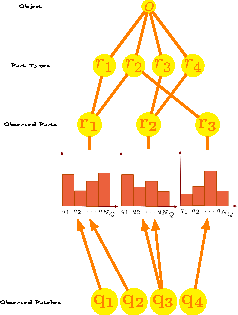
\includegraphics[width=0.7\textwidth]{rel.pdf}
\end{center}
\caption{A schematic diagram of the developed compositional model, for one object class $o$. For each object, the observed patches 
$\mathbf{Q}=\{\mathbf{q_1},\ldots,\mathbf{q_4}\}$ are matched to the patch 
codebook $Q=\{q_1,\ldots,q_{N_{Q}}\}$. An object part is represented as a 
histogram of patch types. An object from class $o$ consists of a set of parts 
$\mathbf{R}=\{\mathbf{r_1},\mathbf{r_2},\mathbf{r_3}\}$ which are matched to the 
part codebook $R=\{r_1,\ldots,r_{N_{R}}\}$. For enabling object recognition, we 
learn the probabilities $p(r_1,\ldots,r_{N_{R}} \vert o)$ as well as part 
connectivity based on the boundary patches $p(q_{1},q_{2} \vert o)$.} 
\label{fig:rel}
\end{figure}

The novelty of our approach is two-fold. First, the proposed algorithm forms semantically meaningful object parts in a hierarchical manner, by exploiting the object functionality, and more specifically in our case the object graspability. Next, it provides a generalization mechanism for recognizing novel object instances, by exploiting the relations between adjacent parts, where the composition at each level of the hierarchy is learned from grasping experience.

We evaluated our method on our collected Ikea Object Dataset \cite{website} and on the RGB-D Washington dataset \cite{rgbd-dataset}. Our approach achieved promising results, outperforming competing methods \cite{rel7}.

%More details can be found in Annexes \ref{ann:icra} and \ref{ann:cvpr}.
More details can be found in Sec.~\ref{ann:icra} and~\ref{ann:cvpr}. %, available at~\href{./attachedPapers/rezapouretal-cvpr2015.pdf}{this link} and~\href{./attachedPapers/rezapouretal-icra2015.pdf}{this link}, respectively.


\subsubsection{Task 2.1 Integrating haptics into 3D compositional models}

The aim of Task 2.1 consists of integrating non-visual features into the 3D 
compositional model.

To achieve the objectives of Task 2.1, we have taken several steps. First, we 
implemented a framework for acquiring tactile information simultaneously with 
visual data, using our robotic framework. 

Next, we recorded a dataset of Ikea objects, consisting of RGB and depth data, 
grasping information and tactile readings corresponding to the grasped patches 
of the object. In these experiments we used a parametrization suitable for our 
Schunk hand. In order to find a good parametrization of tactile features, we 
have done a pre-analysis of the acquired data, by extracting a set of features 
such as object diameter, compressibility, standard deviation of intensity values 
and translation and rotation invariant Chebyshev moments and using a multi-class 
SVM classifier. The details of the developed method are included in Sec.~\ref{ann:techReportKiechle}. The results of the analysis showed that our 
approach was useful for object discrimination using only non-visual features. 
Therefore, we will use a similar tactile feature parametrization and associate 
it with our developed 3D compositional model for obtaining a multi-modal 
representation.

Furthermore, using our developed compositional framework presented in Task 2.3 
and described in detail in Sec.~\ref{ann:cvpr}, we decompose an object into its 
constituent parts and associate the corresponding tactile features. The 
integration of visual and non-visual features is done in a probabilistic manner, 
as described in the technical report included in Sec.~\ref{ann:techReport}. One 
application of the proposed representation is object class recognition in case 
of partial or missing sensory data, either visual or non-visual.

The actual steps required for extracting tactile features and fusing them with 
visual features are:

\begin{enumerate}

\item Extract features from the tactile readings.
\item Associate the extracted features to the part level of the hierarchy.
\item Formulate in a probabilistic manner the binding of haptic and visual features.
\item Propagate the visual and non-visual information in the
  hierarchy, in a bottom-up manner, to allow inference of one type of
  information in the absence of the other.
\end{enumerate}

\comment{[MP] New details will be added under this section, based on the input received from Pisa and from one of our students.}

\subsubsection{Task 2.2 Integrating graspability into 3D compositional models}

In this Task, we associated grasps to object parts, obtained using our proposed 
compositional framework. This approach facilitates grasping unknown objects, 
which are composed of parts similar to those learned by our hierarchical model. 
To facilitate this task, we have designed and implemented a compositional 
framework which is described in detail in Sec.~\ref{ann:cvpr}. The description 
of the grasp representation and of the experimental setup is presented in Sec.~\ref{ann:techReportAlex}.
%, available at~\href{./attachedPapers/rietzeler-techReport.pdf}{this link}.

The steps performed to associate grasps to object parts are:
\begin{enumerate}
\item Record a dataset of grasped object parts, by capturing object relative wrist pose of the gripper, tactile signature and kinesthetic signature (gripper joints).
\item Detect and localize object parts using our proposed compositional model introduced in Task 2.3.
\item Form a set of 3D shape templates according to different grasp types (pinch, spherical, and parallel).
\item Given a scene, align the set of 3D shape templates to the cropped point-cloud sections, provided by the part recognition module and chose the best one according to an optimization procedure.
\item Evaluate the association of grasps to object parts, by performing robotic experiments on a test set containing objects partially similar to the ones in the training set.
\end{enumerate}

The grasp template alignment procedure is based on our pose estimation algorithm~\cite{detry2010ac}, where the 6D pose dependent cross correlation between the shape distribution of the scene and a template is computed.

Next, in order to find a single best grasp for each template, we have developed a grasp inference algorithm which searches over a large number of hypothesis, while performing collision checking with the environment and checking inverse kinematics reachability of the gripper wrist pose hypothesis.

The performed experiments show the obtained grasp association score is of 70\%, 
while the prediction of successful from unsuccessful grasps based on haptic 
features achieves an average accuracy of 80\%. The discussion of the 
experimental results is included in Sec~\ref{ann:techReportAlex}.

\subsubsection{Task 2.4 3D compositional models of the work space}

Reasoning about a scene can be very useful for action planning or grasp planning in the presence of clutter. Visual information plays the most important role, while additional information such as object graspability and non-visual features such as haptics, can be also useful for obtaining an improved and refined representation of the work space.

Therefore, we have analyzed first the performance of our developed 3D compositional model mainly on two aspects: part recognition for novel objects 
and object classification and localization. A detailed description of the method 
and the achieved results can be found in Task 2.3, while we present next a brief 
discussion of our main contributions.

Due to the compositionality nature of our object representationin which object 
parts are described by the relationship between sub-parts, which are 
subsequently represented based on the relationships between small adjacent 
patches, we were able to obtain a high average recognition rate of 85\% on novel 
object instances, composed of parts different from the ones in the training set. 
The generalization property of our model is due to the fact that we learn the 
relations between adjacent parts in an object and therefore our method is not 
fully dependant on the structure of a part. Furthermore, our approach 
outperformed state-of-the-art methods \cite{vfh}, which achieved poor results 
for novel object instances.

Next, we enriched the representation of a scene, by associating grasp templates to detected object parts, as described in Task 2.2.

Finally, as future work we plan to analyze the stability of a grasp using haptic information which can indicate to what extent the test grasp configuration is similar to training data.

\subsection{Relation to the state-of-the-art}

The main contribution of the results achieved for Task 2.3 lies in a successful design and implementation of a learnt compositional hierarchy. The main 
difference from other works \cite{rel2,comp2} introducing hierarchical 
compositional 3D object models, consists in the generalization and scale 
invariant properties of our representation. 

Furthermore, by exploiting the relations between object parts, we were able to 

recognize novel object instances having a similar structure, while the local 
appearance of a part was different from the learned examples. Our method 
achieved an accuracy of 85\% for the recognition of novel object instances, 
outperforming state-of-the-art methods \cite{vfh}. 

Moreover, our proposed method performed better at decomposing an object into 
parts, compared with \cite{rel7}, where the notion of object convexity and 
concavity was exploited for segmenting an object into parts.

In the state-of-the-art methods for part-based object recognition 
\cite{part2,part3,part1}, parts are manually labeled in the training examples, 
while the novelty of our approach consists in extracting the region 
corresponding to a part, from grasping experiments. An object is grasped in 
different ways, depending on its intended functionality, information which is 
exploited in our framework for forming semantically meaningful parts.

\newpage

\bibliographystyle{IEEEtran}
\bibliography{../shared_bibliography/abbreviations,./bibliography/DR21}

\newpage

\appendix

\section{Annexes}

%Which papers / articles are included in the report? Mention titles, authors, publication info; abstract; and a one-liner relating the publication back to the discussion on actual work performed.

\subsection{Article: Learning 3D Object Parts through Grasping} \label{ann:icvs}
\begin{description}
	\item[Authors] Safoura Rezapour Lakani, Mirela Popa, Antonio J. Rodriguez-Sanchez and Justus Piater
	\item[Info] in preparation to be submitted to the 10th International Conference on Computer Vision Systems (ICVS), 2015
	\item[Abstract] Most objects are composed of parts which have a semantic 
meaning. A handle can have many different shapes and be present in quite 
different objects, but there is only one semantic meaning to a handle, which is 
"a part that is designed especially to be grasped by the hand". We introduce 
here a novel 3D algorithm for the decomposition of objects into their 
semantically meaningful parts. These meaningful parts are learned from 
experiments where a robot grasps different objects. Object are represented in a 
compositional graph hierarchy where their parts are represented as the 
relationship between sub-parts, which are subsequently represented based on the 
relationships between small adjacent regions. Unlike other 2D compositional 
approaches, the importance of our 3D oriented method relies on the relationship 
between adjacent regions and sub-parts and where the composition at each level 
of the hierarchy is learned from grasping experience. We evaluate the validity 
of our compositional approach in three different scenarios, where we test the 
importance of the extracted relationships, its robustness to scale and more 
importantly, the recognition of parts from previously unseen objects
	\item[Relation with the deliverable] The paper addresses Task 2.3 by introducing a method for learning objects parts 
in a bottom-up way, from robotic experiments of grasping objects

    \item[Attachment] (following pages until next annex)
\end{description}
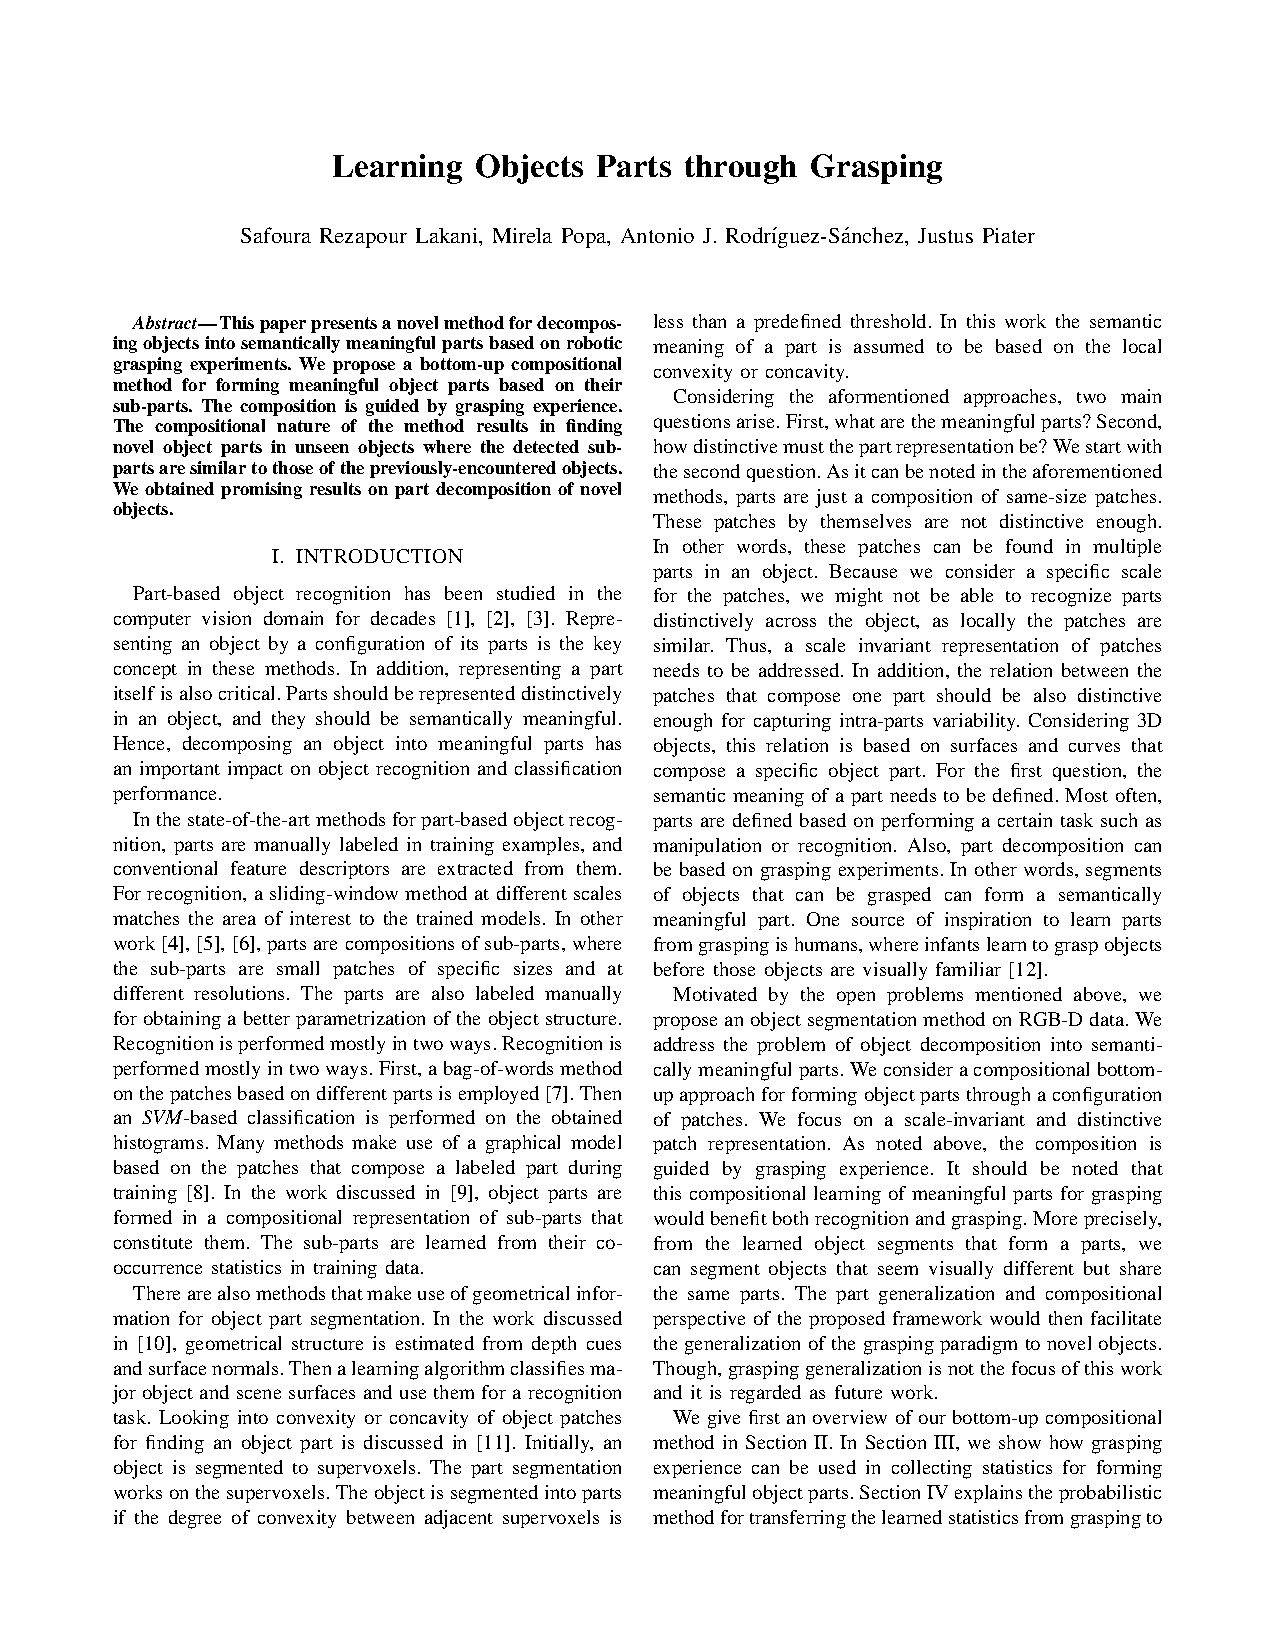
\includepdf[pages=-]{./attachedPapers/rezapouretal-icra2015.pdf}

\subsection{Article: Learning Part-Based 3D Compositional Object Representations} \label{ann:cvpr}
\begin{description}
	\item[Authors] Safoura Rezapour Lakani, Antonio J. Rodriguez-Sanchez and Justus Piater
	\item[Info] submitted to IEEE Computer Vision and Pattern Recognition (CVPR), 2015.
	\item[Abstract] This paper presents a novel approach to parts-based object 
representation from depth images. We propose a bottom-up compositional model for 
representing object classes. Our model uses a probabilistic approach to build 
object representations starting from small patches that are successively built 
up into regions, and finally meaningful (possibly graspable) parts . Parts 
represented this way are the main representatives of the identity of an object 
class. We have evaluated our method at parts recognition and object 
categorization, outperforming competing methods
	\item[Relation with the deliverable] The paper presents a probabilistic model for learning object representations in a hierarchical manner. This representation is useful for all the tasks, as it 
enables forming objects by graspability (Task 2.3), it allows integration of 
non-visual features (Task 2.1), and it can be used for a refined scene 
description (Task 2.4)
    \item[Attachment] (following pages until next annex)
\end{description}
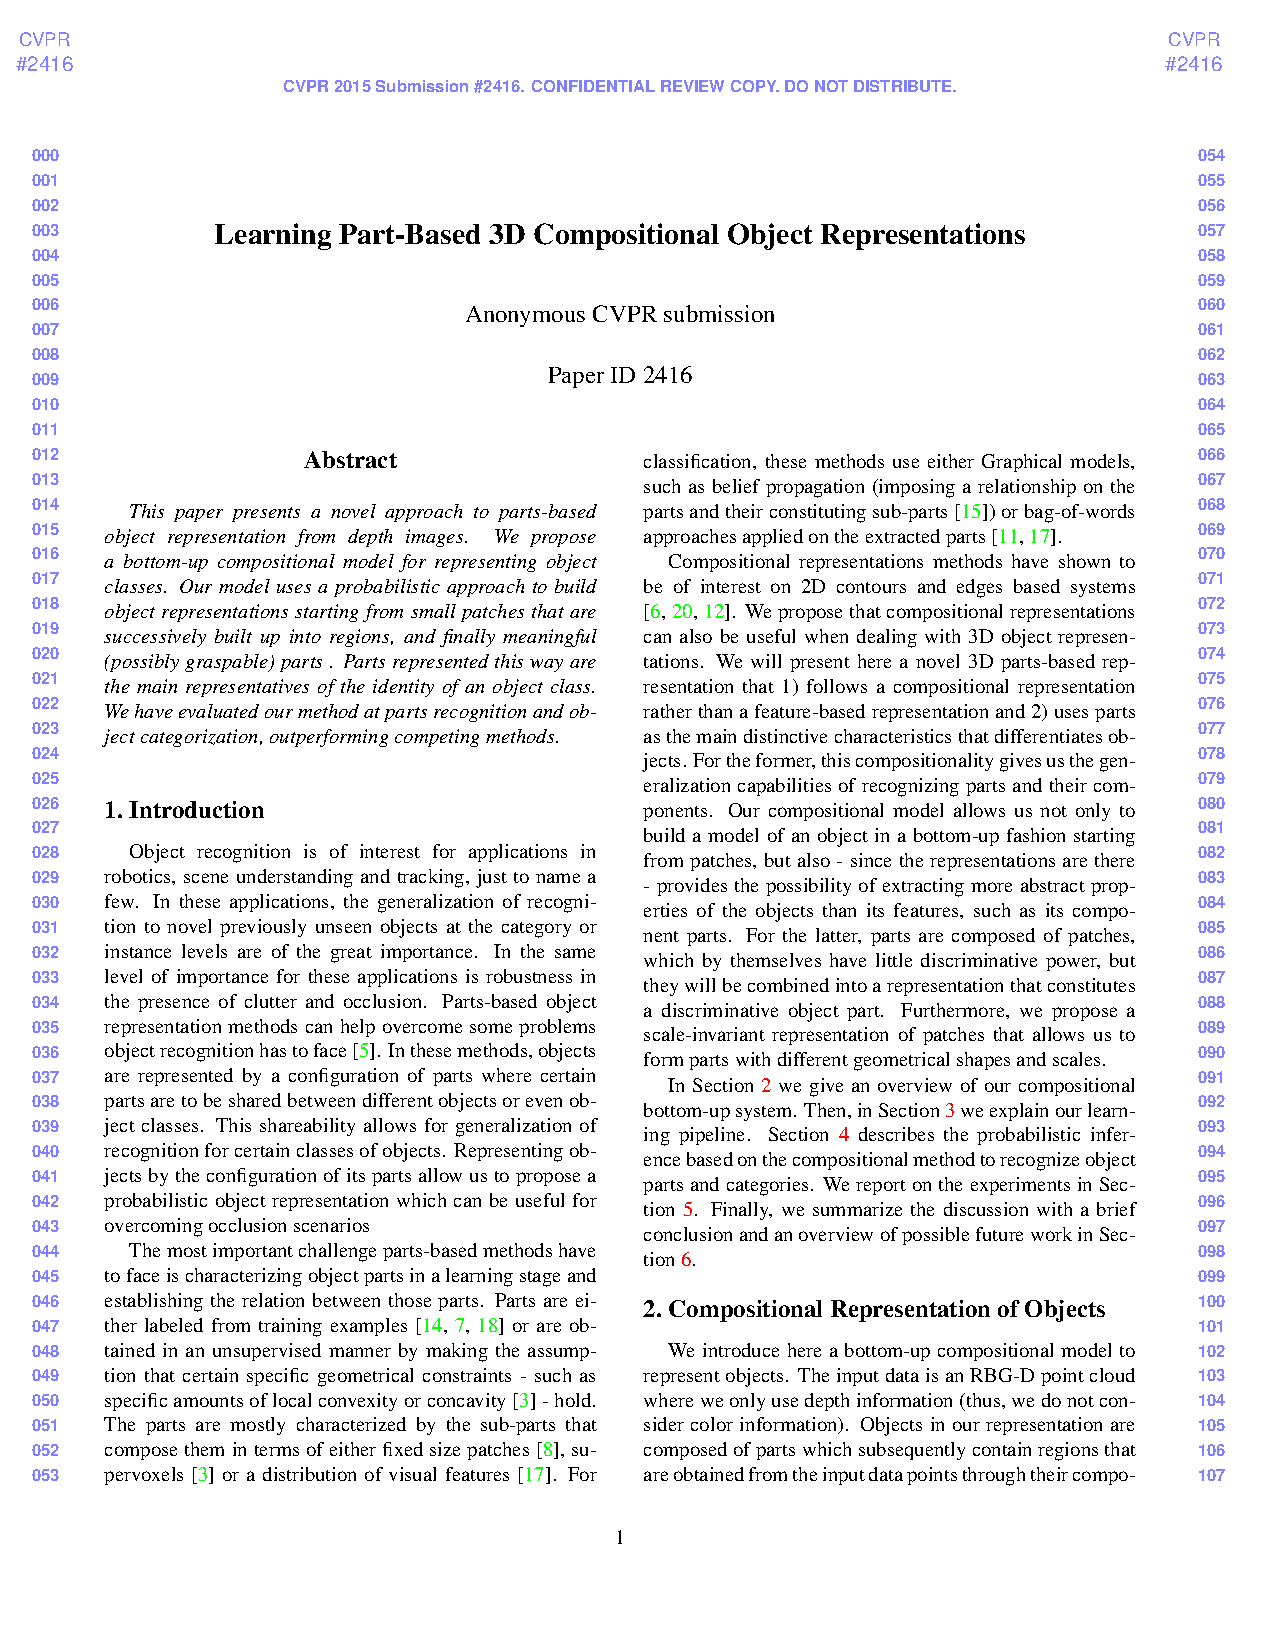
\includepdf[pages=-]{./attachedPapers/rezapouretal-cvpr2015.pdf}

\subsection{Technical Report: Multi-Modal Compositional Object Representation} \label{ann:techReport}
\begin{description}
\item[Authors] Safoura Rezapour Lakani and Justus Piater
\item[Info] Internal technical report
\item[Abstract] The objective of this technical report is to introduce an 
object representation based on both visual and non-visual features such as 
haptics features. The multi-modal representation will allow us to infer visual 
information based on haptics information and vice-versa. The non-visual features 
are useful at object recognition in case of missing or incomplete visual 
observations. We have developed a 3D compositional part-based object 
representation, where the non-visual features are represented by tactile 
information after grasping an object

\item[Relation with the deliverable] The technical report introduces a method for associating grasp templates to 
object parts obtained using the 3D compositional model presented in Task 2.3
\item[Attachment] (following pages until next annex)
\end{description}
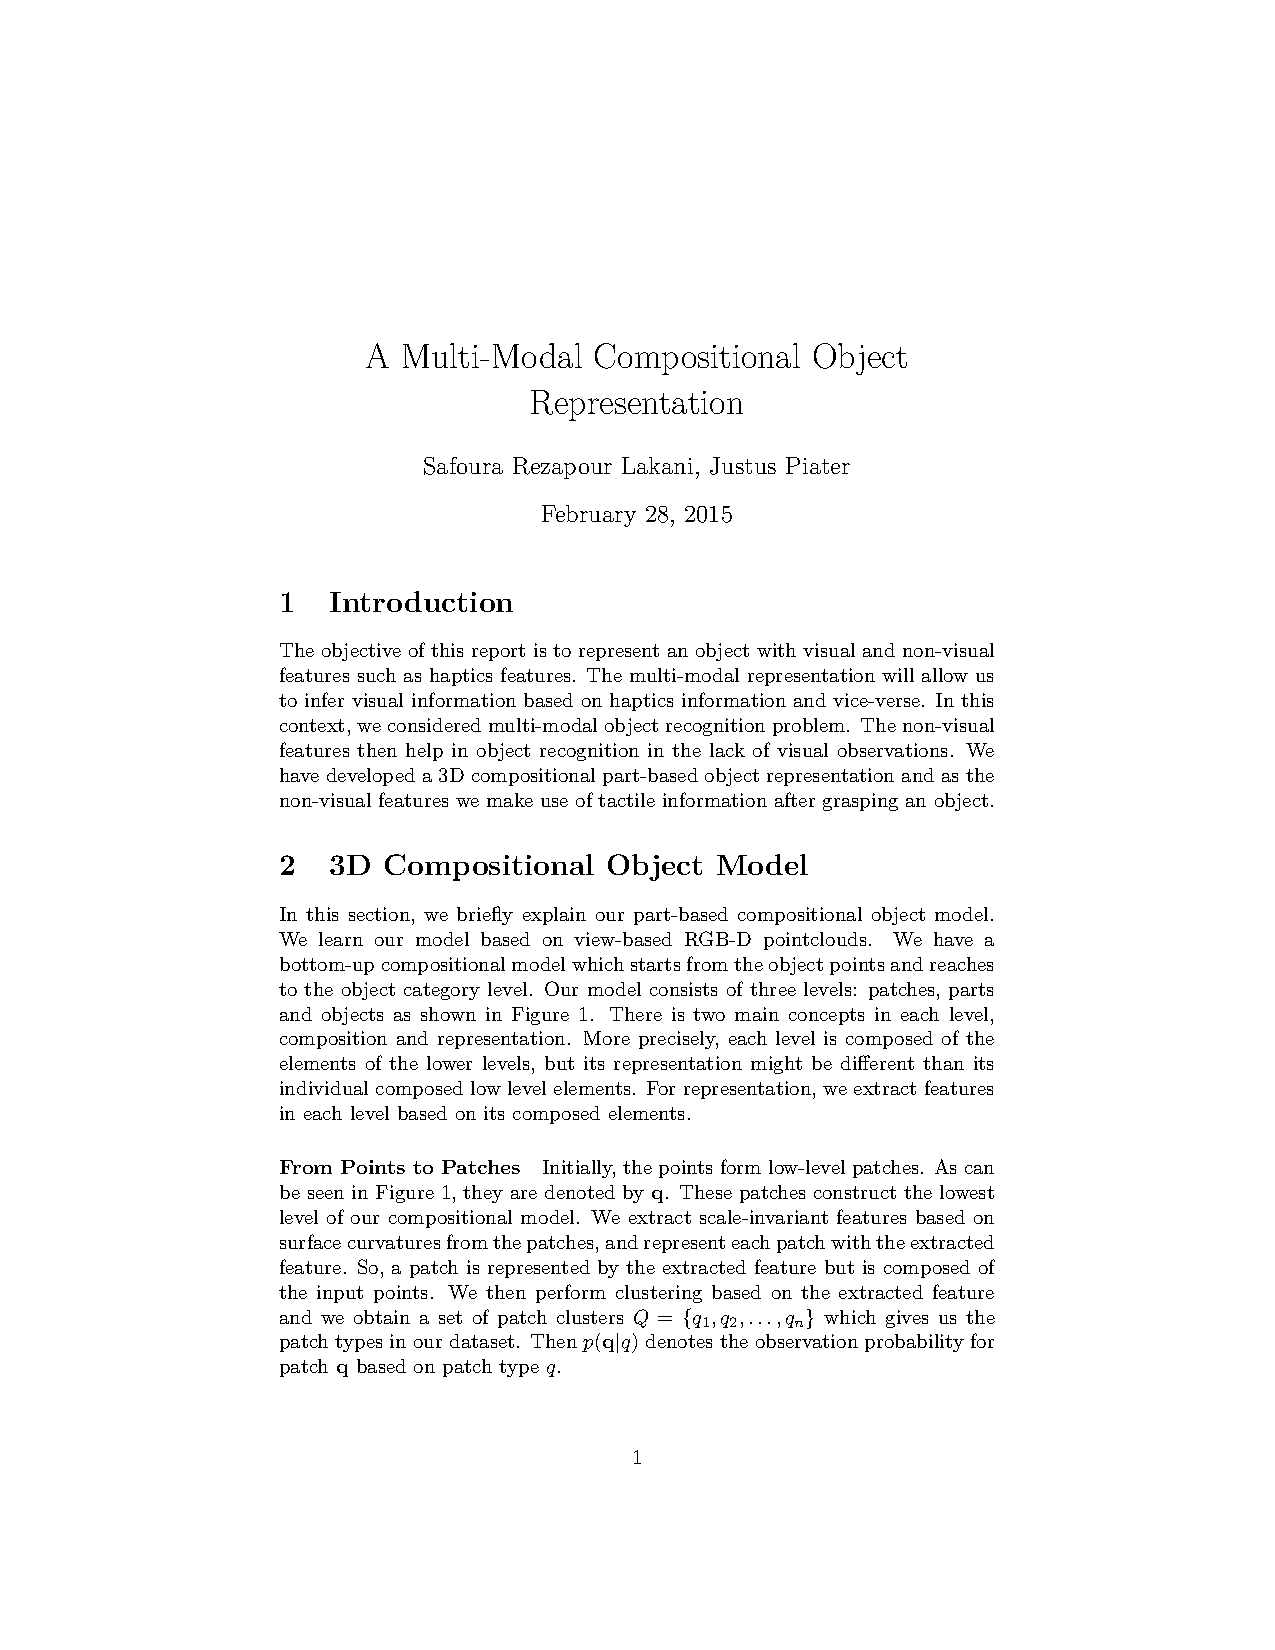
\includepdf[pages=-]{./attachedPapers/rezapouretal-Tech2015.pdf}

\subsection{Technical Report: 3D Compositional Model associated with Grasp Templates and Haptic Data} \label{ann:techReportAlex}
\begin{description}
\item[Authors] Alexander Rietzler
\item[Info] Internal technical report
\item[Abstract] The objective of this technical report is to associate 
graspability and haptic characteristics to object parts produced by a 3D 
compositional model. The advantage of the proposed method resides in the ability 
to perform robust grasping of novel object instances, composed of parts similar 
to the ones existing in the training set
\item[Relation with the deliverable] The technical report introduces a method for associating grasp templates to object parts obtained using the 3D compositional model presented in Task 2.3
\item[Attachment] (following pages)
\end{description}
\includepdf[pages=-]{./attachedPapers/rietzler-techReport.pdf}

\subsection{Technical Report: Object classification using tactile sensor information} \label{ann:techReportKiechle}
\begin{description}
\item[Authors] Peter Kiechle
\item[Info] Internal technical report
\item[Abstract] he objective of this technical report is to describe the 
tactile data acquistion procedure using our robotic framework. Next, it presents 
a parametrization of haptic information, by extracting a set of features such as 
object diameter, compressibility, standard deviation of intensity values and 
translation and rotation invariant Chebyshev moments. Finally, it presents an 
analysis of the obtained results, showing that the proposed method is useful for 
object discrimination
\item[Relation with the deliverable] TThe technical report introduces a method for parametrizing haptic features and 
analyzes its performance for object discrimination. This analysis is useful for 
Task 2.1, in which a similar tactile feature parametrization will be associated 
with our developed 3D compositional model for obtaining a multi-modal 
representation
\item[Attachment] (following pages)
\end{description}
\includepdf[pages=-]{./attachedPapers/kiechle-techReport.pdf}

\end{document}
